\documentclass[11pt,a4paper]{article}
\usepackage[T1]{fontenc}
\usepackage[utf8]{inputenc}
\usepackage{lmodern,amsmath,amssymb,geometry,xcolor,hyperref,booktabs,tabularx,tikz,fancyhdr,enumitem}
\renewcommand{\tablename}{Tabla}
\renewcommand{\figurename}{Figura}
\renewcommand{\contentsname}{Índice}
\renewcommand{\refname}{Referencias}
\usetikzlibrary{arrows.meta}
\geometry{left=22mm,right=22mm,top=23mm,bottom=22mm}

% Paleta de colores compartida según el plan técnico
\definecolor{tinta}{HTML}{17313A}
\definecolor{verde}{HTML}{096A57}
\definecolor{azul}{HTML}{205C9C}
\definecolor{oro}{HTML}{B58A42}
\definecolor{gris}{HTML}{51656D}
\definecolor{fondo}{HTML}{EAF4EF}
\definecolor{alerta}{HTML}{AE403A}

\hypersetup{
  colorlinks=true,
  urlcolor=azul,
  linkcolor=verde,
  citecolor=azul,
  pdftitle={Laberintos y rutas alternativas - Proyecto 1},
  pdfsubject={Modelación de red dirigida, caminos mínimos, flujo unitario y corte mínimo},
  pdfauthor={Cristian Cáceres, Ariel Díaz, Gustavo Martínez, Sebastián Mena},
  pdflang={es-CL}
}

\renewcommand{\familydefault}{\sfdefault}
\color{tinta}
\setlength{\parindent}{0pt}
\setlength{\parskip}{6pt}
\setlength{\headheight}{14pt}
\setlength{\emergencystretch}{2em}
\renewcommand{\arraystretch}{1.22}
\setlist[enumerate]{leftmargin=6mm,itemsep=2pt,topsep=3pt}

\pagestyle{fancy}
\fancyhf{}
\fancyhead[L]{\small\color{gris}INFO1158 / Teoría de Grafos}
\fancyhead[R]{\small\color{gris}Laberintos y rutas alternativas}
\fancyfoot[R]{\small\color{verde}\thepage}
\renewcommand{\headrulewidth}{.3pt}

\newcommand{\tema}[1]{\subsection*{\color{verde}#1}}
\newcommand{\ruta}[1]{\textcolor{verde}{\ensuremath{#1}}}
\newcommand{\alternativa}[1]{\textcolor{azul}{\ensuremath{#1}}}

\begin{document}

% ==============================================================================
% PORTADA INSTITUCIONAL
% ==============================================================================
\begin{titlepage}
\thispagestyle{empty}
\vspace*{5mm}
{\small\bfseries\color{gris}TEORÍA DE GRAFOS \ \textbar\ \ INFO1158}\par
\vspace{2mm}
{\color{oro}\rule{\linewidth}{1.5pt}}\par
\vspace{18mm}

{\fontsize{28}{32}\selectfont\bfseries\color{tinta} Laberintos y\\rutas alternativas\par}
\vspace{8mm}
{\large\bfseries\color{verde} Proyecto 1 $\cdot$ Informe técnico}\par
\vspace{4mm}
{\color{gris}\normalsize Modelación de una red dirigida, caminos mínimos, alternativas independientes y cortes de pasillos para inspección logística.}\par

\vspace{16mm}
\begin{center}
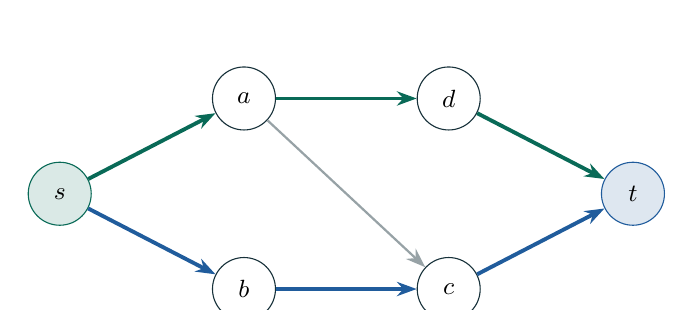
\begin{tikzpicture}[x=1.3cm,y=1.1cm,
  n/.style={circle,draw=tinta,fill=white,minimum size=8mm,inner sep=0pt,font=\small\bfseries},
  a/.style={-{Stealth[length=2.5mm,width=1.8mm]},draw=tinta!45,line width=.8pt}]
  \node[n,fill=verde!15,draw=verde] (s) at (0,1.2) {$s$};
  \node[n] (a) at (1.8,2.3) {$a$};
  \node[n] (b) at (1.8,0.1) {$b$};
  \node[n] (d) at (3.8,2.3) {$d$};
  \node[n] (c) at (3.8,0.1) {$c$};
  \node[n,fill=azul!15,draw=azul] (t) at (5.6,1.2) {$t$};
  \draw[a,draw=verde,line width=1.4pt] (s) -- (a);
  \draw[a,draw=azul,line width=1.4pt] (s) -- (b);
  \draw[a] (a) -- (c);
  \draw[a,draw=verde,line width=1.4pt] (a) -- (d);
  \draw[a,draw=azul,line width=1.4pt] (b) -- (c);
  \draw[a,draw=azul,line width=1.4pt] (c) -- (t);
  \draw[a,draw=verde,line width=1.4pt] (d) -- (t);
\end{tikzpicture}
\end{center}

\vfill

\begin{minipage}[t]{0.55\linewidth}
  \textbf{\color{verde}Integrantes} \small (Equipo autorizado de cuatro)\\[1.5mm]
  Cristian Cáceres\\
  Ariel Díaz\\
  Gustavo Martínez\\
  Sebastián Mena
\end{minipage}
\begin{minipage}[t]{0.42\linewidth}
  \textbf{\color{verde}Docente}\\[1.5mm]
  Elliott Mardones Arias\\[4mm]
  \textbf{\color{verde}Fecha de entrega}\\[1.5mm]
  26 de noviembre de 2026
\end{minipage}
\vspace{4mm}
{\color{oro}\rule{\linewidth}{1.2pt}}
\end{titlepage}

% ==============================================================================
% ÍNDICE GENERAL
% ==============================================================================
\newpage
\pagenumbering{roman}
\thispagestyle{plain}
{
  \hypersetup{linkcolor=tinta}
  \tableofcontents
}
\newpage
\pagenumbering{arabic}

% ==============================================================================
% SECCIÓN 1: INTRODUCCIÓN
% ==============================================================================
\section{Introducción}

La teoría de grafos permite modelar y optimizar sistemas discretos en los que interesa caracterizar la conectividad, la transitabilidad y la robustez estructural ante contingencias. En informática e ingeniería logística, este marco se aplica al diseño de redes de comunicación, gestión de dependencias y ruteo automatizado~\cite{cormen,sedgewick}. El presente proyecto aborda la operación de robots autónomos de inspección en un centro de almacenamiento organizado mediante pasillos de sentido único~\cite{enunciado}.

Cada misión de inspección parte desde una entrada designada $s$ y concluye en una salida $t$, respetando estrictamente la orientación de cada pasillo. La distancia se define como la cantidad de pasillos recorridos (arcos), abstrayendo variaciones de longitud métrica para concentrar el análisis en las propiedades topológicas del laberinto.

El problema formula tres interrogantes fundamentales interconectadas:
\begin{enumerate}
  \item \textbf{Eficiencia de tránsito:} ¿Cuál es el camino que utiliza la menor cantidad de pasillos entre $s$ y $t$?
  \item \textbf{Redundancia e independencia:} ¿Cuántas rutas dirigidas pueden operar simultáneamente sin compartir ningún arco, asegurando que el bloqueo de un pasillo no inhabilite a varias trayectorias a la vez?
  \item \textbf{Vulnerabilidad y corte:} ¿Cuál es el conjunto mínimo de pasillos que, al quedar inhabilitados, interrumpe por completo todo desplazamiento desde la entrada hasta la salida?
\end{enumerate}

Para responder a estos objetivos, se modela la red mediante un grafo dirigido, se investigan y contrastan formalmente algoritmos de búsqueda (BFS frente a DFS) y de caminos disjuntos (enumeración exhaustiva frente a flujo unitario con Edmonds--Karp), y se verifica la equivalencia matemática entre el número máximo de rutas independientes y la cardinalidad del corte mínimo.

El desarrollo se contrasta empíricamente a través de una red base de 11 vértices y 18 arcos, sobre la cual se analizan dos modificaciones operativas (el bloqueo de un pasillo y la habilitación de un atajo), un caso de desconexión total y un caso manual independiente de 6 vértices diseñado para trazar la cancelación residual. Los resultados se respaldan mediante una suite automatizada de pruebas unitarias y un script reproducible de verificación.

% ==============================================================================
% SECCIÓN 2: PARTE TEÓRICA
% ==============================================================================
\newpage
\section{Parte teórica}

\subsection{Modelo dirigido y objetivos del análisis}
Una red de almacenamiento se representa como un grafo dirigido $G = (V, E)$, donde el conjunto de vértices $V$ corresponde a intersecciones o áreas de trabajo y el conjunto de arcos $E$ modela los pasillos transitables desde un origen $u$ hacia un destino $v$, denotados como pares ordenados $(u, v)$. Un arco activo se encuentra habilitado para el tráfico; bloquear un pasillo equivale a excluirlo temporalmente de la adyacencia activa sin destruir su registro en el inventario de la red.

Para cualquier camino dirigido $P = (s = v_0, v_1, \dots, v_k = t)$, su longitud se define como la cantidad de arcos $|E(P)| = k$. La distancia mínima $d_G(s, t)$ es la menor longitud entre todas las rutas posibles:
\[
  d_G(s, t) = \min \{ |E(P)| : P \text{ es un camino dirigido de } s \text{ a } t \text{ en } G \}.
\]
Si la salida $t$ es inalcanzable desde $s$, se establece expresamente la ausencia de ruta, evitando asignar distancias numéricas artificiales como cero.

Una familia de caminos $\mathcal{P} = \{P_1, P_2, \dots, P_k\}$ es \emph{disjunta en arcos} (o independiente) si ningún par comparte conexiones:
\[
  E(P_i) \cap E(P_j) = \varnothing \quad \forall i \neq j.
\]
Esta condición permite que las rutas compartan vértices intermedios, pero prohíbe terminantemente la concurrencia en un mismo pasillo.

Por su parte, un \emph{corte de pasillos} es un subconjunto de arcos $C \subseteq E$ cuya supresión elimina todo camino dirigido entre la entrada y la salida en el grafo residual $G - C = (V, E \setminus C)$. El problema de corte mínimo busca minimizar la cardinalidad $|C|$.

\subsection{Búsqueda de un camino: BFS y DFS}
Para determinar la existencia de un camino entre $s$ y $t$, existen dos estrategias canónicas de exploración: Breadth-First Search (BFS) y Depth-First Search (DFS)~\cite{cormen,mitocw}.

\begin{center}
{\small
\begin{tabularx}{\linewidth}{@{}p{.22\linewidth}XX@{}}
\toprule
\textbf{Estrategia} & \textbf{Estructura y exploración} & \textbf{Garantía de camino obtenido} \\
\midrule
BFS (Anchura) & Cola FIFO; explora por capas concéntricas de distancia creciente. & \textbf{Óptimo}: garantiza el camino con el menor número de arcos en grafos no ponderados. \\
DFS (Profundidad) & Pila (LIFO) o recursión; avanza por una rama hasta agotar alternativas. & \textbf{No óptimo}: el camino depende del orden de adyacencia y puede ser arbitrariamente largo. \\
\bottomrule
\end{tabularx}}
\end{center}

\textbf{Justificación de la selección:} Se selecciona **BFS**. Al procesar la frontera mediante una cola FIFO, el algoritmo descubre los vértices en orden estricto de distancia: ningún vértice situado a distancia $d+1$ es extraído antes de que se hayan procesado todos los vértices a distancia $d$. Al almacenar para cada nodo su predecesor inmediato, la ruta mínima se reconstruye desde $t$ hacia $s$ y se invierte en tiempo lineal. Con listas de adyacencia, la complejidad temporal es $O(|V| + |E|)$ y la memoria auxiliar es $O(|V|)$~\cite{cormen}.

\subsection{Familia máxima mediante enumeración exhaustiva}
La primera alternativa para calcular el máximo número de caminos disjuntos en arcos consiste en generar exhaustivamente todos los caminos dirigidos simples entre $s$ y $t$ y resolver el problema combinatorio de selección de subconjuntos compatibles~\cite{sedgewick}.

\tema{Generación de candidatos con retroceso (backtracking)}
Se inicia una exploración DFS desde $s$. Para evitar ciclos infinitos y rutas redundantes, se mantiene un conjunto de vértices presentes en el camino actual (\texttt{visitados\_en\_camino}). A diferencia de un DFS estándar que marca vértices de forma global e irreversible, el retroceso remueve el vértice de la marca al terminar la exploración de sus ramas salientes. Esto permite que un mismo vértice pueda figurar en distintos caminos candidatos sin omitir alternativas válidas.

Basta considerar caminos simples: si un trayecto contiene un ciclo dirigido, eliminar dicho ciclo conserva los extremos $s$ y $t$ reduciendo los arcos utilizados. Por ende, la eliminación de ciclos nunca perjudica la compatibilidad con otros caminos.

\tema{Selección de la mayor familia compatible}
Obtenidos los $P$ caminos simples candidatos, cada camino $P_i$ se asocia a su conjunto de arcos $E(P_i)$. El algoritmo evalúa las $2^P$ combinaciones posibles mediante búsqueda exhaustiva o ramificación y poda:
\begin{enumerate}
  \item Para cada camino candidato, se evalúa la decisión binaria de incluirlo o descartarlo.
  \item La inclusión solo es factible si $E(P_i) \cap \bigcup_{P \in \mathcal{P}_{\text{parcial}}} E(P) = \varnothing$.
  \item Se conserva la familia factible de mayor cardinalidad.
\end{enumerate}

\tema{Contraejemplo: Por qué la estrategia voraz falla}
Una aproximación voraz (*greedy*) que seleccione un camino mínimo y bloquee inmediatamente sus arcos no garantiza la solución óptima. Consideremos el grafo manual con candidatos:
\[
  P_0 = s \to a \to c \to t, \quad P_1 = s \to a \to d \to t, \quad P_2 = s \to b \to c \to t.
\]
Si se elige vorazmente $P_0$ (longitud 3), se consumen los arcos $(s, a)$ y $(c, t)$. Esto inhabilita tanto a $P_1$ como a $P_2$, dejando una familia de tamaño 1. En cambio, descartar $P_0$ permite seleccionar la familia $\{P_1, P_2\}$, cuya cardinalidad es 2. La enumeración exhaustiva garantiza el máximo porque explora todas las combinaciones, pero su costo temporal es exponencial en el peor caso ($O(2^P)$), volviéndola impracticable en redes de escala productiva.

\subsection{Flujo unitario y algoritmo de Edmonds–Karp}
La segunda alternativa modela el problema como una red de flujo dirigida en la que cada arco activo posee capacidad unitaria $c(u, v) = 1$~\cite{cormen,edmondskarp}.

Un flujo admisible $f: E \to \mathbb{R}$ debe satisfacer dos axiomas:
\begin{align}
  0 \le f(u, v) \le 1 & \quad \forall (u, v) \in E \quad &\text{(Restricción de capacidad)}, \\
  \sum_{u:(u,v) \in E} f(u, v) = \sum_{w:(v,w) \in E} f(v, w) & \quad \forall v \in V \setminus \{s, t\} \quad &\text{(Conservación en nodos intermedios)}.
\end{align}
El valor del flujo $|f|$ representa la cantidad neta que egresa de $s$. Al fijar capacidades unitarias, la restricción asegura que ningún arco pueda ser utilizado por más de un camino.

\tema{Red residual: corrección mediante arcos inversos}
La red residual $G_f = (V, E_f)$ modela la capacidad disponible para reorganizar el flujo. Para cada arco original $(u, v) \in E$:
\begin{itemize}
  \item Posee una capacidad directa residual $c_f(u, v) = 1 - f(u, v)$, que permite aumentar el flujo si está libre.
  \item Posee una capacidad inversa residual $c_f(v, u) = f(u, v)$, que permite cancelar asignaciones previas si el arco ya transporta flujo.
\end{itemize}
Recorrer un arco inverso $(v, u)$ en la red residual no significa que un robot viaje físicamente en sentido contrario en el almacén; representa la operación algebraica de deshacer una asignación provisional anterior para canalizarla hacia un destino alternativo, posibilitando que dos rutas independientes converjan hacia la solución global óptima.

\tema{Procedimiento de Edmonds–Karp seleccionado}
El algoritmo implementa el método de Ford–Fulkerson seleccionando en cada iteración el camino de aumento con menor cantidad de arcos mediante BFS sobre la red residual~\cite{edmondskarp,zeh}:
\begin{enumerate}
  \item Se inicializa el flujo nulo en todos los arcos ($f(u, v) = 0$).
  \item Se ejecuta BFS desde $s$ sobre los arcos residuales con $c_f > 0$.
  \item Si se alcanza $t$, se reconstruye el camino de aumento. En capacidad unitaria, el cuello de botella es 1. Se suma 1 al flujo de cada arco recorrido (restando 1 a su capacidad residual directa y sumando 1 a su inversa).
  \item Se repite hasta que no exista camino dirigido entre $s$ y $t$ en $G_f$.
  \item Se recupera el flujo entero y se descomponen los arcos con $f(u, v) = 1$ en una familia de caminos disjuntos mediante búsquedas encadenadas, descartando posibles circulaciones cerradas~\cite{cormen}.
\end{enumerate}

\textbf{Complejidad:} Al ser capacidades unitarias, si el valor del flujo máximo es $k$, se efectúan exactamente $k$ aumentos exitosos y una búsqueda final de terminación. Cada exploración BFS cuesta $O(|V| + |E|)$. La fase de flujo y extracción toma $O((k+1)(|V| + |E|))$, donde $k \le \min(\delta^+(s), \delta^-(t))$. La cota general asintótica en redes generales es $O(|V||E|^2)$~\cite{cormen}.

\subsection{Relación entre caminos independientes y corte mínimo}
El fundamento teórico central del proyecto descansa en el teorema de flujo máximo y corte mínimo formulado por Ford y Fulkerson, estrechamente vinculado al Teorema de Menger para grafos dirigidos~\cite{cormen,zeh}.

\begin{center}
\colorbox{fondo}{
\begin{minipage}{0.92\linewidth}
\vspace{2mm}
\centering
\textbf{Relación fundamental de dualidad en el proyecto:}
\[
  \underbrace{\text{Máximo de caminos disjuntos}}_{\text{Rutas independientes concurrentes}} = \underbrace{|f_{\max}|}_{\text{Flujo unitario}} = \underbrace{\min |C|}_{\text{Pasillos mínimos a bloquear}}
\]
\vspace{1mm}
\end{minipage}}
\end{center}

\tema{Deducción constructiva del corte desde la red residual}
Cuando Edmonds–Karp finaliza, no existe camino de aumento hacia $t$. Sea $S \subset V$ el conjunto de vértices alcanzables desde $s$ mediante arcos con capacidad residual positiva ($c_f > 0$). Por definición de parada, $t \notin S$. El corte de pasillos $C$ se define como el conjunto de arcos dirigidos originales activos que parten de $S$ y llegan al conjunto complementario $V \setminus S$:
\[
  C = \{ (u, v) \in E : u \in S, \ v \notin S \}.
\]
Propiedades matemáticas del corte resultante:
\begin{enumerate}
  \item \textbf{Saturación:} Cada arco $(u, v) \in C$ tiene $f(u, v) = 1$. Si tuviera $f(u, v) = 0$, su capacidad residual directa sería $1 - 0 = 1 > 0$, lo que implicaría que $v$ sería alcanzable desde $u \in S$, contradiciendo que $v \notin S$.
  \item \textbf{Flujo entrante nulo:} Cualquier arco original $(w, z)$ con $w \notin S$ y $z \in S$ debe tener $f(w, z) = 0$. De lo contrario, existiría un arco inverso en la residual con capacidad $f(w, z) = 1$ desde $z \in S$ hacia $w$, haciendo que $w \in S$.
  \item \textbf{Igualdad exacta:} Al sumar la conservación de flujo sobre todos los nodos de $S$, los flujos internos se cancelan y se obtiene $|f| = \sum_{e \in C} f(e) = |C|$.
\end{enumerate}
Por tanto, la cardinalidad de la familia disjunta extraída coincide rigurosamente con el tamaño del corte de pasillos hallado, certificando matemáticamente la optimalidad simultánea de ambos resultados.

\begin{center}
{\small
\begin{tabularx}{\linewidth}{@{}p{.22\linewidth}XX@{}}
\toprule
\textbf{Criterio} & \textbf{Enumeración exhaustiva} & \textbf{Flujo unitario (Edmonds--Karp)} \\
\midrule
Certificado de optimalidad & Por exploración completa del espacio $2^P$. & Por dualidad con el corte mínimo ($|f_{\max}| = |C|$). \\
Reconsideración de pasos & Mediante retroceso sistemático (*backtracking*). & Mediante arcos residuales inversos. \\
Espacio de búsqueda & Requiere generar todos los caminos simples. & No necesita enumerar caminos; opera sobre la red residual. \\
Corte mínimo obtenido & Requiere un algoritmo de corte independiente. & Se obtiene de forma constructiva desde el conjunto $S$. \\
Idoneidad en la app & Útil para contraste en redes pequeñas. & **Seleccionado**: polinómico, escalable y robusto. \\
\bottomrule
\end{tabularx}}
\end{center}

% ==============================================================================
% SECCIÓN 3: DESARROLLO APLICADO DEL PROYECTO
% ==============================================================================
\newpage
\section{Desarrollo aplicado del proyecto}

\subsection{Construcción y validación del modelo inicial}
El centro de almacenamiento inicial se modela mediante el grafo dirigido $G_0 = (V, E_0)$, conformado por 11 vértices y 18 arcos activos:
\[
  V = \{s, A, B, C, D, E, F, G, H, I, t\}, \quad |V| = 11, \quad |E_0| = 18.
\]

\begin{center}
\small
\begin{tabular}{cl@{\hspace{14mm}}cl}
\toprule
\textbf{Vértice origen} & \textbf{Destinos activos} & \textbf{Vértice origen} & \textbf{Destinos activos} \\
\midrule
$s$ & $A, B, C$ & $F$ & $I$ \\
$A$ & $D, E$    & $G$ & $E, H$ \\
$B$ & $E, F$    & $H$ & $I$ \\
$C$ & $G, H$    & $I$ & $t$ \\
$D$ & $t, F$    & $t$ & $\varnothing$ \\
$E$ & $D, H$    &     & \\
\bottomrule
\end{tabular}
\end{center}

\begin{center}
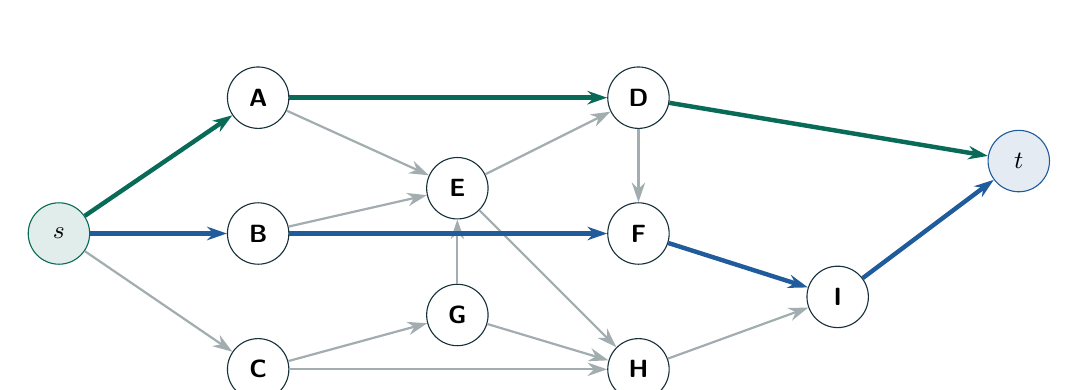
\begin{tikzpicture}[x=1.15cm,y=1.15cm,
  n/.style={circle,draw=tinta,fill=white,minimum size=7.8mm,inner sep=0pt,font=\small\bfseries},
  a/.style={-{Stealth[length=2.5mm,width=1.7mm]},draw=tinta!40,line width=.8pt}]
  \node[n,fill=verde!12,draw=verde] (s) at (0,1.6) {$s$};
  \node[n] (A) at (2.2,3.1) {A};
  \node[n] (B) at (2.2,1.6) {B};
  \node[n] (C) at (2.2,.1) {C};
  \node[n] (E) at (4.4,2.1) {E};
  \node[n] (G) at (4.4,.7) {G};
  \node[n] (D) at (6.4,3.1) {D};
  \node[n] (F) at (6.4,1.6) {F};
  \node[n] (H) at (6.4,.1) {H};
  \node[n] (I) at (8.6,.9) {I};
  \node[n,fill=azul!12,draw=azul] (t) at (10.6,2.4) {$t$};
  \foreach \u/\v in {s/C,A/E,B/E,C/G,C/H,D/F,E/D,E/H,G/E,G/H,H/I} {\draw[a] (\u) -- (\v);}
  \foreach \u/\v in {s/A,A/D,D/t} {\draw[a,draw=verde,line width=1.6pt] (\u) -- (\v);}
  \foreach \u/\v in {s/B,B/F,F/I,I/t} {\draw[a,draw=azul,line width=1.6pt] (\u) -- (\v);}
\end{tikzpicture}\par
\vspace{2mm}
{\small\color{gris}\textbf{Figura 1.} Red inicial de almacenamiento $G_0$. Verde: ruta mínima $s \to A \to D \to t$. Azul: ruta alternativa independiente $s \to B \to F \to I \to t$.}
\end{center}

\textbf{Validación de restricciones del enunciado:}
\begin{itemize}[noitemsep]
  \item \textbf{Dimensiones iniciales:} Satisface $10 \le |V| = 11 \le 12$ y $14 \le |E_0| = 18 \le 20$.
  \item \textbf{Integridad de arcos:} Sin lazos reflexivos ($u \neq v$), pares ordenados únicos (sin arcos múltiples) y sin arcos recíprocos o antiparalelos ($(u,v) \in E_0 \implies (v,u) \notin E_0$).
  \item \textbf{Conectividad:} Ningún vértice está aislado; todos poseen grado incidente $\ge 1$.
  \item \textbf{Certificado inicial de alternativas:} Los caminos $P_1 = s \to A \to D \to t$ y $P_2 = s \to B \to F \to I \to t$ son disjuntos en arcos, certificando un mínimo de dos rutas independientes concurrentes.
\end{itemize}

\subsection{Resolución de la red original}
La aplicación de BFS desde $s$ sobre $G_0$ construye las capas de distancia:
\[
  L_0 = \{s\}, \quad L_1 = \{A, B, C\}, \quad L_2 = \{D, E, F, G, H\}, \quad L_3 = \{t, I\}.
\]
El predecesor de $t$ es $D$, el de $D$ es $A$, y el de $A$ es $s$. Se reconstruye la ruta mínima \ruta{s \to A \to D \to t}, de longitud $d=3$. Dado que ningún vecino directo de $s$ conecta con $t$, no existen rutas de longitud 1 ni 2.

El análisis de flujo máximo obtiene un valor de 2 rutas disjuntas, descomponibles en $P_1$ y $P_2$. Los vértices residuales alcanzables son $S = \{s, A, B, C, D, E, F, G, H\}$. El corte saliente hacia $V \setminus S = \{I, t\}$ resulta $C_0 = \{ (D, t), (I, t) \}$, con cardinalidad 2. La igualdad $|f_{\max}| = |C_0| = 2$ confirma la optimalidad de la solución.

\subsection{Modificaciones y análisis comparativo}
Para estudiar la respuesta de la red ante contingencias operativas, se contrastan dos modificaciones introducidas de forma independiente sobre $G_0$, conservando los mismos extremos $s$ y $t$:

\begin{center}
{\small
\begin{tabularx}{\linewidth}{@{}p{.23\linewidth}ccp{.25\linewidth}cX@{}}
\toprule
\textbf{Configuración} & \textbf{Arcos} & \textbf{$d$} & \textbf{Camino mínimo} & \textbf{$k$} & \textbf{Corte mínimo ($C$)} \\
\midrule
Red original $G_0$ & 18 & 3 & $s \to A \to D \to t$ & 2 & $\{(D,t), (I,t)\}$ \\
Bloqueo $D \to t$  & 17 & 4 & $s \to B \to F \to I \to t$ & 1 & $\{(I,t)\}$ \\
Atajo $C \to t$    & 19 & 2 & $s \to C \to t$ & 3 & $\{(s,A), (s,B),$ $(s,C)\}$ \\
\bottomrule
\end{tabularx}}
\end{center}

\tema{Bloqueo de pasillo: Menor redundancia de rutas y mayor distancia}
Al inhabilitar el pasillo $D \to t$, el único arco de acceso a la salida pasa a ser $I \to t$. Como alcanzar $I$ demanda al menos 3 arcos, la nueva distancia mínima se incrementa a $d=4$ a través de $s \to B \to F \to I \to t$. Toda ruta dirigida debe converger obligatoriamente por el pasillo $I \to t$; en consecuencia, la familia disjunta se reduce drásticamente a $k=1$, y el corte mínimo queda conformado únicamente por $C_1 = \{(I, t)\}$ ($|C_1|=1$). La red sigue conectada (pues existe ruta alternativa para $D$ mediante $D \to F \to I \to t$), pero pierde su redundancia operativa.

\tema{Incorporación de un atajo: Menor distancia y mayor redundancia}
Al agregar el pasillo directo $C \to t$, se genera la ruta ultracorta $s \to C \to t$ de longitud $d=2$, óptima dado que no existe arco $s \to t$. Al combinarse con las rutas previas $P_1$ y $P_2$, es posible transportar simultáneamente $k=3$ rutas disjuntas en arcos:
\[
  P_1 = s \to A \to D \to t, \quad P_2 = s \to B \to F \to I \to t, \quad P_3 = s \to C \to t.
\]
El corte mínimo asciende a tamaño 3. Puede representarse bloqueando todas las salidas de $s$, $C_2 = \{(s, A), (s, B), (s, C)\}$, o todas las entradas de $t$, $C_2' = \{(D, t), (I, t), (C, t)\}$, demostrando que el corte mínimo puede no ser único.

\subsection{Caso manual: contraste de las estrategias}
Se diseña un caso independiente de 6 vértices y 7 arcos para seguir la traza paso a paso:
\[
  V_m = \{s, a, b, c, d, t\}, \quad E_m = \{(s,a), (s,b), (a,c), (a,d), (b,c), (c,t), (d,t)\}.
\]

\begin{center}
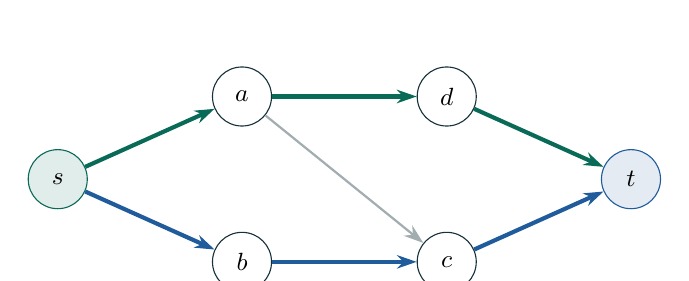
\begin{tikzpicture}[x=1.3cm,y=1.05cm,
  n/.style={circle,draw=tinta,fill=white,minimum size=7.5mm,inner sep=0pt,font=\small\bfseries},
  a/.style={-{Stealth[length=2.5mm,width=1.7mm]},draw=tinta!40,line width=.8pt}]
  \node[n,fill=verde!12,draw=verde] (s) at (0,1.2) {$s$};
  \node[n] (a) at (1.8,2.2) {$a$};
  \node[n] (b) at (1.8,0.2) {$b$};
  \node[n] (d) at (3.8,2.2) {$d$};
  \node[n] (c) at (3.8,0.2) {$c$};
  \node[n,fill=azul!12,draw=azul] (t) at (5.6,1.2) {$t$};
  \draw[a,draw=verde,line width=1.5pt] (s) -- (a);
  \draw[a,draw=azul,line width=1.5pt] (s) -- (b);
  \draw[a] (a) -- (c);
  \draw[a,draw=verde,line width=1.5pt] (a) -- (d);
  \draw[a,draw=azul,line width=1.5pt] (b) -- (c);
  \draw[a,draw=azul,line width=1.5pt] (c) -- (t);
  \draw[a,draw=verde,line width=1.5pt] (d) -- (t);
\end{tikzpicture}\par
\vspace{2mm}
{\small\color{gris}\textbf{Figura 2.} Caso manual independiente. El arco central $a \to c$ permite ilustrar la cancelación residual.}
\end{center}

\tema{Traza algorítmica: dos aumentos y una cancelación residual}
\begin{enumerate}
  \item \textbf{Estado inicial:} Flujo $f(e) = 0$ en los 7 arcos.
  \item \textbf{Primer aumento:} BFS encuentra el camino de menor orden lexicográfico $P_0 = s \to a \to c \to t$ (longitud 3). Se saturan con flujo 1 los arcos $(s, a)$, $(a, c)$ y $(c, t)$. En la red residual, se habilitan los arcos inversos $(a, s)$, $(c, a)$ y $(t, c)$.
  \item \textbf{Segundo aumento con cancelación:} La siguiente búsqueda BFS sobre la red residual encuentra la trayectoria de aumento:
  \[
    s \longrightarrow b \longrightarrow c \stackrel{\text{inverso}}{\longrightarrow} a \longrightarrow d \longrightarrow t.
  \]
  El paso por el arco inverso residual $(c, a)$ **cancela** la unidad de flujo previa en el arco original $(a, c)$, reduciendo su flujo neto de 1 a 0.
  \item \textbf{Estado final:} Los arcos con flujo neto 1 se descomponen limpiamente en las dos rutas independientes $P_1 = s \to a \to d \to t$ y $P_2 = s \to b \to c \to t$.
\end{enumerate}

\begin{center}
{\small
\begin{tabular}{lccc}
\toprule
\textbf{Arco original} & \textbf{Flujo inicial} & \textbf{Tras 1.er aumento ($P_0$)} & \textbf{Tras 2.º aumento (Cancelación)} \\
\midrule
$s \to a$ & 0 & 1 & \textbf{1} \\
$s \to b$ & 0 & 0 & \textbf{1} \\
$a \to c$ & 0 & 1 & \textbf{\color{alerta}0 (Cancelado)} \\
$a \to d$ & 0 & 0 & \textbf{1} \\
$b \to c$ & 0 & 0 & \textbf{1} \\
$c \to t$ & 0 & 1 & \textbf{1} \\
$d \to t$ & 0 & 0 & \textbf{1} \\
\bottomrule
\end{tabular}}
\end{center}

\subsection{Verificación matemática y contraste con el código}
Se implementó el script reproducible \texttt{verificar\_informe.py}, el cual evalúa las 5 configuraciones mediante el cliente de pruebas interno de Flask (\texttt{app.test\_client()}) y ejecuta de forma paralela la enumeración exhaustiva de caminos simples con retroceso.

\begin{center}
{\small
\begin{tabularx}{\linewidth}{@{}lcccccX@{}}
\toprule
\textbf{Configuración} & \textbf{Activos} & \textbf{Caminos simples} & \textbf{Distancia ($d$)} & \textbf{Flujo ($k$)} & \textbf{Corte} & \textbf{Estado} \\
\midrule
Original               & 18 & 14 & 3 & 2 & 2 & Validado con certificado \\
Bloqueo $D \to t$      & 17 & 10 & 4 & 1 & 1 & Validado con certificado \\
Atajo $C \to t$        & 19 & 15 & 2 & 3 & 3 & Validado con certificado \\
Caso manual            & 7  & 3  & 3 & 2 & 2 & Validado con certificado \\
Sin conexión           & 16 & 0  & Sin ruta & 0 & 0 & Desconexión validada \\
\bottomrule
\end{tabularx}}
\end{center}

En el caso sin conexión (bloqueo simultáneo de $D \to t$ e $I \to t$), el motor devuelve \texttt{ruta: null}, \texttt{distancia: null}, \texttt{caminos: []}, \texttt{maximo: 0} y \texttt{corte: []}. El corte vacío certifica que en la red ya modificada no es necesario bloquear ningún pasillo adicional para impedir el tránsito. Los resultados completos se registran en el archivo estructurado \texttt{verificacion-resultados.json}.

% ==============================================================================
% SECCIÓN 4: IMPLEMENTACIÓN Y REPRODUCCIÓN
% ==============================================================================
\newpage
\section{Implementación y reproducción}

\subsection{Organización del código y correspondencia algorítmica}
La solución se desarrolló en Python 3 utilizando Flask para la capa de servicios web, implementando los algoritmos mediante estructuras de datos nativas (\texttt{list}, \texttt{dict}, \texttt{set} y \texttt{collections.deque}), sin recurrir a bibliotecas externas de teoría de grafos como NetworkX.

\begin{center}
{\small
\begin{tabularx}{\linewidth}{@{}p{.26\linewidth}X@{}}
\toprule
\textbf{Módulo / Archivo} & \textbf{Responsabilidad técnica} \\
\midrule
\texttt{casos.json} & Almacena las redes base reproducibles (caso original y caso manual). \\
\texttt{modelo.py} & Carga y validación: rechaza lazos, arcos múltiples y recíprocos; valida límites de $|V|$ y $|E|$. \\
\texttt{algoritmos.py} & Implementa \texttt{bfs}, \texttt{flujo\_unitario}, descomposición de rutas y corte desde alcanzables residuales. \\
\texttt{app.py} & Expone los servicios HTTP (\texttt{GET /}, \texttt{GET /casos/<id>} y \texttt{POST /analizar}). \\
\texttt{templates/}, \texttt{static/} & Interfaz de usuario: plano SVG dirigido, edición interactiva y visualización de soluciones. \\
\texttt{tests/} & Suite de 16 pruebas automatizadas con \texttt{unittest} cubriendo modelo, algoritmos y API. \\
\texttt{verificar\_informe.py} & Script de reproducibilidad que valida los 5 casos y ejecuta la enumeración exhaustiva. \\
\bottomrule
\end{tabularx}}
\end{center}

\subsection{Interacción y contrato de análisis}
La comunicación cliente-servidor se rige por un contrato JSON estricto mediante la ruta \texttt{POST /analizar}. La petición transfiere el estado completo: \texttt{vertices}, \texttt{entrada}, \texttt{salida} y la lista de \texttt{arcos} con su propiedad booleana \texttt{activo}.

La respuesta entrega:
\begin{itemize}[noitemsep]
  \item \texttt{ruta}: lista ordenada de vértices del camino mínimo (o \texttt{null}).
  \item \texttt{distancia}: entero que indica la cantidad de pasillos utilizados (o \texttt{null}).
  \item \texttt{caminos}: lista de listas de vértices correspondientes a la familia máxima disjunta.
  \item \texttt{maximo}: cardinalidad de la familia de rutas independientes ($|f_{\max}|$).
  \item \texttt{corte}: lista de arcos $[u, v]$ que conforman el corte mínimo saliente del conjunto $S$.
\end{itemize}

La interfaz web incorpora una barra de controles que permite alternar dinámicamente entre la vista normal y el resaltado visual sobre el plano SVG: verde para el camino mínimo, azul y oro para las rutas disjuntas, y rojo punteado para el corte mínimo.

\subsection{Guía de instalación y reproducción}
El código fuente está disponible en el repositorio oficial del proyecto:\\
\url{https://github.com/SebasMenas/TeoriaGrafosTrabajo}

\textbf{Pasos de ejecución (Linux / macOS / PowerShell):}
\begin{verbatim}
# 1. Crear y activar entorno virtual
python3 -m venv .venv
source .venv/bin/activate       # En Windows: .\.venv\Scripts\activate

# 2. Instalar dependencias
pip install -r requirements.txt

# 3. Ejecutar suite de pruebas unitarias
python3 -m unittest discover -s tests -v

# 4. Ejecutar script de verificación y enumeración matemática
python3 verificar_informe.py

# 5. Iniciar la aplicación web
flask --app app run
\end{verbatim}
La aplicación interactiva queda accesible localmente en \url{http://127.0.0.1:5000}.

% ==============================================================================
% SECCIÓN 5: CONCLUSIONES (PÁGINA EXCLUSIVA)
% ==============================================================================
\clearpage
\section{Conclusiones}

El desarrollo del proyecto permitió analizar y modelar computacionalmente el comportamiento de robots de inspección en un entorno de almacenamiento dirigido, respondiendo satisfactoriamente a las tres interrogantes planteadas en la formulación del problema.

\tema{Divergencia entre caminos combinatorios y redundancia real}
Un hallazgo conceptual determinante consiste en la marcada diferencia entre la cantidad total de caminos simples posibles y el número máximo de alternativas independientes que pueden operar en paralelo. En la red original existen **14 caminos dirigidos simples**, pero únicamente **2 pueden coexistir sin compartir pasillos**. De forma análoga, tras inhabilitar el arco $D \to t$, persisten **10 caminos simples**, pero todos dependen críticamente del único pasillo de entrada restante $I \to t$, reduciendo la redundancia real a 1. Esto demuestra que evaluar la resiliencia de un centro logístico contando simplemente las rutas existentes resulta engañoso: la verdadera robustez operativa está gobernada por la disyunción de arcos y por los cuellos de botella que delimita el corte mínimo.

\tema{Garantías algorítmicas y corrección residual}
Para determinar la ruta de menor longitud en pasillos, la búsqueda en anchura (BFS) demostró ser la estrategia óptima frente a DFS, alcanzando una cota $O(|V| + |E|)$ gracias a la exploración por capas concéntricas.

Para maximizar las rutas alternativas independientes, tanto la enumeración exhaustiva con retroceso como el flujo unitario mediante Edmonds–Karp proporcionan soluciones exactas. No obstante, la enumeración exhaustiva presenta una complejidad exponencial $O(2^P)$ que la vuelve inviable para sistemas dinámicos. En contraste, Edmonds–Karp resuelve el problema en tiempo fuertemente polinómico $O((k+1)(|V| + |E|))$, entregando simultáneamente el certificado matemático del corte mínimo gracias a la dualidad del teorema de flujo máximo y corte mínimo.

El caso de estudio manual demostró de forma concluyente por qué una estrategia voraz fracasa y cuál es la función esencial de la red residual: el uso de arcos residuales inversos no invierte la física del almacén, sino que actúa como un mecanismo algebraico de retroceso que permite deshacer compromisos preliminares subóptimos para alcanzar el óptimo global.

\tema{Alcances del modelo y proyecciones de ingeniería}
El modelo implementado asume pasillos de longitud métrica uniforme y capacidad unitaria, garantizando que dos misiones no colisionen dentro de un mismo arco. Sin embargo, en un almacén físico real, las rutas independientes obtenidas pueden compartir vértices intermedios, lo que podría generar interferencias o tiempos de espera si los robots coinciden simultáneamente en una misma intersección.

Como extensiones futuras para robustecer la aplicación logística, se proyecta:
\begin{enumerate}
  \item Modelar caminos disjuntos en vértices mediante técnicas de desdoblamiento de nodos ($v_{\text{in}} \to v_{\text{out}}$).
  \item Asignar pesos asociados al tiempo de tránsito real o distancias físicas en metros, resolviendo caminos mínimos mediante el algoritmo de Dijkstra.
  \item Incorporar ventanas de tiempo (*Time-Expanded Graphs*) para gestionar de manera integral el tráfico multi-agente en tiempo real.
\end{enumerate}

% ==============================================================================
% SECCIÓN 6: REFERENCIAS (COMPACTA Y FORMAL)
% ==============================================================================
\clearpage
\section{Referencias}

{\small
\begin{enumerate}[label={[\arabic*]},itemsep=4pt,topsep=2pt,leftmargin=7mm]
  \bibitem{enunciado} INFO1158 (2026). \emph{Proyecto 1: Simulador interactivo de laberintos y rutas alternativas}. Escuela de Informática, Universidad Católica de Temuco. Guía docente y rúbricas de evaluación, pp.~1--5.

  \bibitem{cormen} Cormen, T.~H., Leiserson, C.~E., Rivest, R.~L. y Stein, C. (2022). \emph{Introduction to Algorithms}, 4.\,a edición. The MIT Press. Cap.~20 (Elementary Graph Algorithms: BFS), Cap.~24 (Maximum Flow, Ford-Fulkerson Method, Max-Flow Min-Cut Theorem).

  \bibitem{edmondskarp} Edmonds, J. y Karp, R.~M. (1972). Theoretical Improvements in Algorithmic Efficiency for Network Flow Problems. \emph{Journal of the ACM}, 19(2), pp.~248--264. \href{https://doi.org/10.1145/321694.321699}{doi:10.1145/321694.321699}.

  \bibitem{sedgewick} Sedgewick, R. y Wayne, K. (2011). \emph{Algorithms}, 4.\,a edición. Addison-Wesley Professional. Sección~4.1 (Directed Graphs, Backtracking and AllPaths Enumeration).

  \bibitem{mitocw} Demaine, E., Ku, J. y Solomon, J. (2020). \emph{Introduction to Algorithms (6.006): Lecture 9 (BFS) \& Lecture 10 (DFS)}. MIT OpenCourseWare. \href{https://ocw.mit.edu/courses/6-006-introduction-to-algorithms-spring-2020/}{ocw.mit.edu}.

  \bibitem{zeh} Zeh, N. (2016). \emph{Advanced Graph Algorithms: Edmonds--Karp Algorithm, The Max-Flow Min-Cut Theorem, and Integral Flows}. Faculty of Computer Science, Dalhousie University. Material docente de algoritmos de optimización de redes.

  \bibitem{pallets} Pallets Projects (2024). \emph{Flask Documentation: Quickstart and Application Test Client}. Documentación oficial técnica. \href{https://flask.palletsprojects.com/}{flask.palletsprojects.com}.
\end{enumerate}
}

\end{document}
